\documentclass[english,14pt]{beamer}
\usetheme{EastLansing}
\usecolortheme{spruce}

\usepackage{xcolor}
\usepackage{listings}
\usepackage{courier}
\usepackage{graphicx}
\usepackage{amsmath}
\usepackage{algorithm2e}
\usepackage{multicol}
\usepackage{hyperref}

% http://mirrors.ibiblio.org/CTAN/macros/latex/contrib/datetime2/datetime2.pdf
\usepackage{babel}
\usepackage[useregional]{datetime2}

% https://tex.stackexchange.com/questions/42619/x-mark-to-match-checkmark
\usepackage{pifont}% http://ctan.org/pkg/pifont

%% https://stackoverflow.com/questions/1435837/how-to-remove-footers-of-latex-beamer-templates
%%gets rid of bottom navigation bars
%\setbeamertemplate{footline}[page number]
%
%gets rid of navigation symbols
\setbeamertemplate{navigation symbols}{}


\usefonttheme[onlymath]{serif}

\definecolor{mGreen}{rgb}{0,0.6,0}
\definecolor{mGray}{rgb}{0.5,0.5,0.5}
\definecolor{mPurple}{rgb}{0.8,0,0.82}
\definecolor{backgroundColour}{rgb}{0.95,0.95,0.92}
\definecolor{lightBlue}{rgb}{0.1, 0.1, 0.8}

\newcommand\red[1]{{\color{red} #1}}
\newcommand\green[1]{{\color{green} #1}}
\newcommand\blue[1]{{\color{blue} #1}}

\newcommand{\cmark}{\ding{51}}%
\newcommand{\xmark}{\ding{55}}%

\lstdefinestyle{CStyle}{
    backgroundcolor=\color{backgroundColour},   
    commentstyle=\color{mGreen},
    keywordstyle=\color{magenta},
    numberstyle=\tiny\color{mGray},
    stringstyle=\color{mPurple},
    basicstyle=\footnotesize,
    breakatwhitespace=false,         
    breaklines=true,                 
    captionpos=b,                    
    keepspaces=true,                 
    numbers=left,                    
    numbersep=5pt,                  
    showspaces=false,                
    showstringspaces=false,
    showtabs=false,                  
    tabsize=2,
    language=C
}

\lstdefinestyle{pseudo}{
        basicstyle=\ttfamily\footnotesize,
        keywordstyle=\color{lightBlue},
        morekeywords={BEGIN,END,IF,ELSE,ENDIF,ELSEIF,PRINT,WHILE,RETURN,ENDWHILE,DO,FOR,TO,IN,ENDFOR,BREAK,INPUT},
        morecomment=[l]{//},
        commentstyle=\color{mGreen}
}

\lstset{basicstyle=\footnotesize\ttfamily,breaklines=true}
\lstset{framextopmargin=50pt,tabsize=2}

\title{ENGG1003 - Monday Week 3}
\subtitle{Loops and branching}
\author{Steve Weller}
\institute{University of Newcastle}
%\date{\today}
\date{8 March, 2021}

% following is a bit of a hack, but forces page numbers (technically: frame numbers) to run 1,2,3,... 
% with titlepage counting as frame 1

\addtocounter{framenumber}{1}
\titlepage

\begin{document}

\begin{flushleft}
{\scriptsize Last compiled:~\DTMnow}
\vspace*{-5mm}
\end{flushleft}
\framebreak

%==============================================================

\begin{frame}[fragile]

\frametitle{Lecture overview}
\begin{enumerate}
	\item Iteration using \texttt{for} loop \red{\S3.1}
	\begin{itemize}
		\item fixed number of iterations
%		\item principles
%		\item live demo
	\end{itemize}

	\item[]
	
	\item Iteration using \texttt{while} loop \red{\S3.2}
		\begin{itemize}
			\item keep iterating whenever a condition is satisfied
%			\item principles
%			\item live demo
		\end{itemize}

	\item[]
	
	\item Branching: \texttt{if}, \texttt{elif} and \texttt{else} \red{\S3.3}
		\begin{itemize}
			\item check condition before executing code block
%			\item principles
%			\item live demo
		\end{itemize}
		
\end{enumerate}

\end{frame}

%==============================================================

\begin{frame}[fragile]

\frametitle{$1)$ Iteration using \texttt{for} loop}

\begin{itemize}
	\item many computations are repetitive by nature and programming languages have certain loop structures to deal with this
	\item one such loop structure is the for loop
	\item printing the 5 times table
	\item \textbf{at console---begin with live demo}
\end{itemize}


\end{frame}

%==============================================================

\begin{frame}[fragile]

\frametitle{}

\begin{figure}[ht]
	\centering
	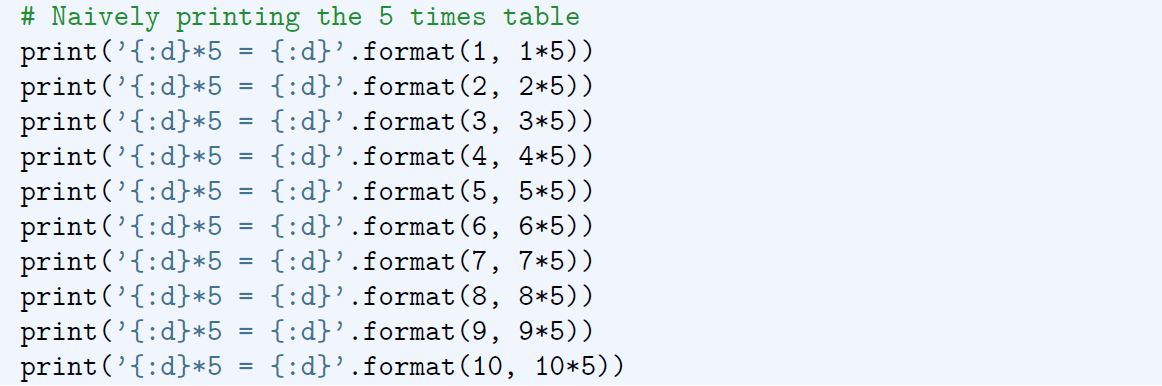
\includegraphics[width=0.8\textwidth]{figures/LLp59}
\end{figure}

\begin{figure}[ht]
	\centering
	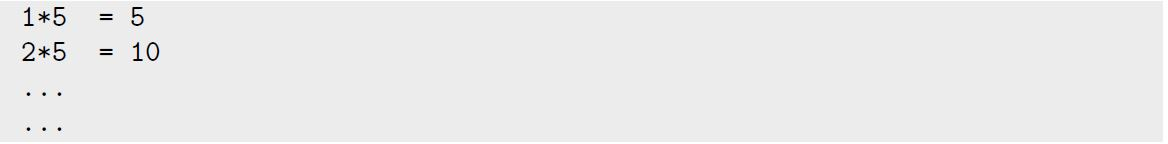
\includegraphics[width=0.8\textwidth]{figures/LLp60a}
\end{figure}
	
\end{frame}

%==============================================================

\begin{frame}[fragile]

\frametitle{}

\begin{itemize}
	\item first loop for i in [1, 2, 3, 4, 5, 6, 7, 8, 9, 10]:
	\item code fragment LLp60
\end{itemize}

\begin{figure}[ht]
	\centering
	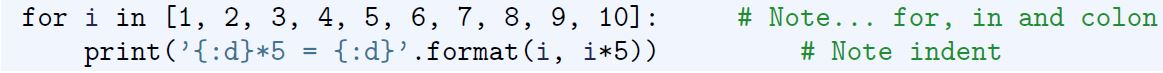
\includegraphics[width=0.8\textwidth]{figures/LLp60b}
\end{figure}

%for i in [1, 2, 3, 4, 5, 6, 7, 8, 9, 10]: # Note... for, in and colon
%print(’{:d}*5 = {:d}’.format(i, i*5)) # Note indent
%With this construction, the loop variable i takes on each of the values 1 to 10, and
%for each value, the print function is called.
%Since the numbers 1 to 10 appear in square brackets, they constitute a special
%structure called a list.

\end{frame}

%==============================================================

\begin{frame}[fragile]

\frametitle{A typical for loop}

\begin{itemize}
	\item general loop structure
	\item indentation---critical!
\end{itemize}

\begin{figure}[ht]
	\centering
	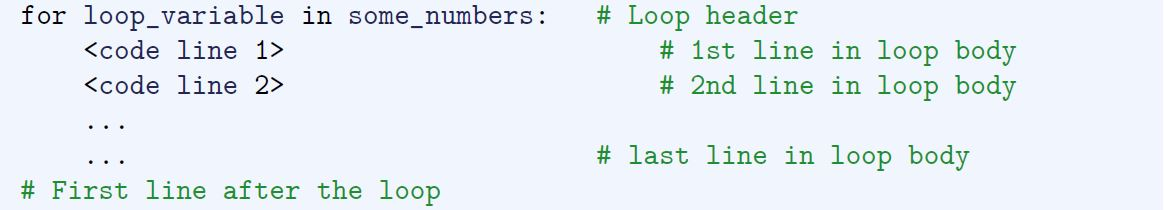
\includegraphics[width=0.8\textwidth]{figures/LLp60c}
\end{figure}


%Loop Structure There are different ways to write for loops, but herein, they are
%typically structured as
%for loop_variable in some_numbers: # Loop header
%<code line 1> # 1st line in loop body
%<code line 2> # 2nd line in loop body
%...
%... # last line in loop body
%# First line after the loop
%where loop_variable runs through the numbers1 given by some_numbers. In the
%very first line, called the for loop header, there are two reserved words, for and
%in. They are compulsory, as is the colon at the end. Also, the block of code lines
%inside a loop must be indented. These indented lines are referred to as the loop body.
%Once the indent is reversed, we are outside (and after) the loop (as commented with
%# First line after the loop, see code). One run-through of the loop body is
%called an iteration, i.e., in our example above with the 5 times table, the loop will
%do 10 iterations.

\end{frame}

%==============================================================

\begin{frame}[fragile]

\frametitle{Nested loops}

%\begin{itemize}
%
%	\item nested loops %? maybe / maybe-not
%\end{itemize}

\begin{figure}[ht]
	\centering
	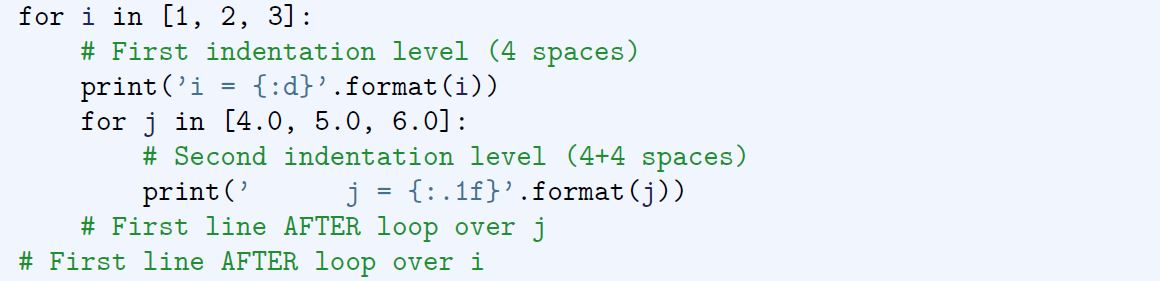
\includegraphics[width=0.8\textwidth]{figures/LLp61a}
\end{figure}

\begin{figure}[ht]
	\centering
	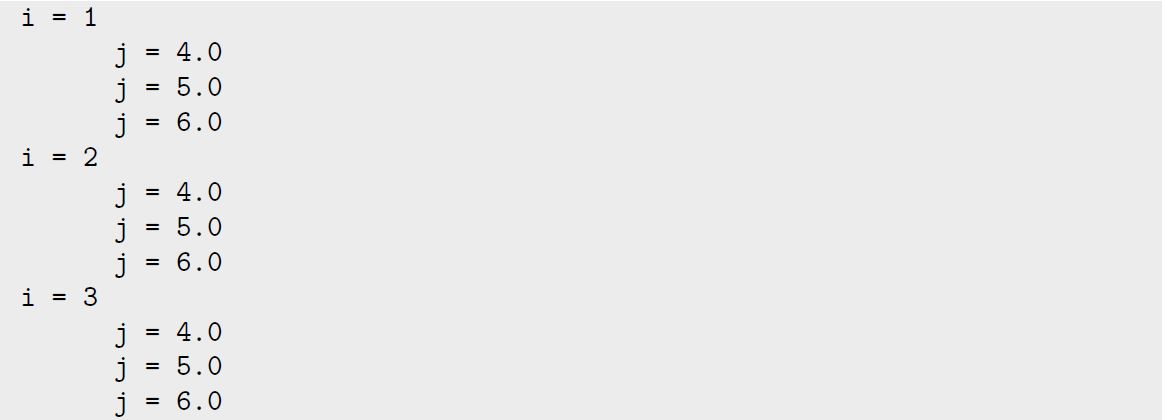
\includegraphics[width=0.8\textwidth]{figures/LLp61b}
\end{figure}

\end{frame}

%==============================================================

\begin{frame}[fragile]

\frametitle{Combining for loop and array}

\begin{itemize}
	\item average height
	\item \S3.1.3
%	\item program on LLp62
\end{itemize}

\begin{figure}[ht]
	\centering
	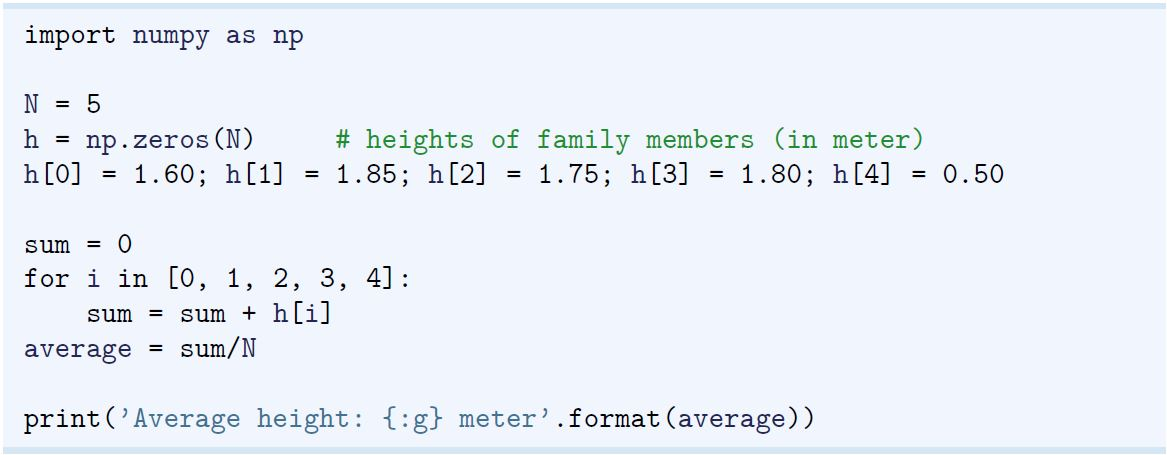
\includegraphics[width=0.8\textwidth]{figures/LLp62a}
\end{figure}

\end{frame}

%==============================================================

\begin{frame}[fragile]

\frametitle{\texttt{range} function}

\begin{itemize}
	\item motivation: 
	\item range(start, stop, step)
	\item eg: range(0,5,1)
	\item why tf the weird indexing?
\end{itemize}

\begin{figure}[ht]
	\centering
	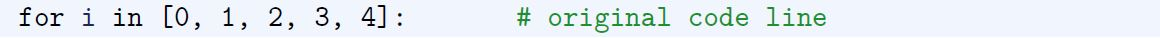
\includegraphics[width=0.8\textwidth]{figures/LLp63a}
\end{figure}

\begin{figure}[ht]
	\centering
	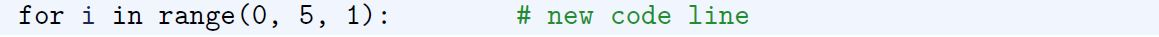
\includegraphics[width=0.8\textwidth]{figures/LLp63b}
\end{figure}

\end{frame}

%==============================================================

\begin{frame}[fragile]

\frametitle{Live demo: for loop}

\begin{itemize}
%	\item run code from \S3.1.3
	\item Python code:~\href{https://github.com/slgit/prog4comp_2/blob/master/py36-src/average_height.py}{\texttt{average\_height.py}}
\end{itemize}

\end{frame}

%==============================================================

\begin{frame}[fragile]

\frametitle{$2)$ Iteration using \texttt{while} loop}

\begin{itemize}
	\item for loop runs for a specified number of iterations
%	\begin{itemize}
%		\item do NOT cover break and continue
%	\end{itemize}
	\item The other basic loop construction in Python is the while loop, which runs as long as a condition is~\texttt{True}

\end{itemize}

\end{frame}

%==============================================================

\begin{frame}[fragile]

\frametitle{Boolean expressions}

	
	
\begin{itemize}
%	\item Boolean type \S2.2.10
%	\item screenshot LLp46, LLp47
%	\item present at the console live demo, then skip over slides
	\item aka \red{\emph{logical expressions}}
	\item these evaluate to \red{\emph{Boolean values}} \texttt{True} and \texttt{False}
	\begin{itemize}
		\item note capital letters T and F
	\end{itemize}
	\item  there are 6 \red{\emph{relational operators}} in Python---comparing values
	 \verb+>, <, >=, <=, ==+ and \verb+!=+
	 \item typeset as simple table
	 %https://www.geeksforgeeks.org/relational-operators-in-python/
	 
\end{itemize}

\end{frame}

%==============================================================

\begin{frame}[fragile]

\frametitle{Relational operators:~comparing values}

Live demo of relational operators

\begin{figure}[ht]
	\centering
	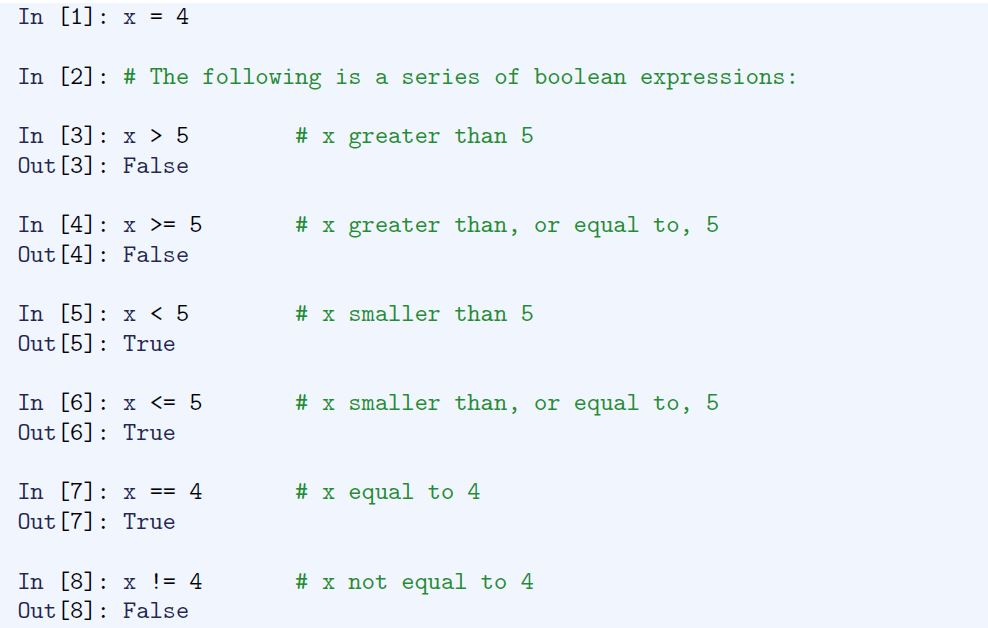
\includegraphics[width=0.8\textwidth]{figures/LLp46}
\end{figure}


	
\end{frame}

%==============================================================

\begin{frame}[fragile]

\frametitle{Boolean operators: \texttt{and}, \texttt{or}, \texttt{not}}

Live demo of Boolean operators

\begin{figure}[ht]
	\centering
	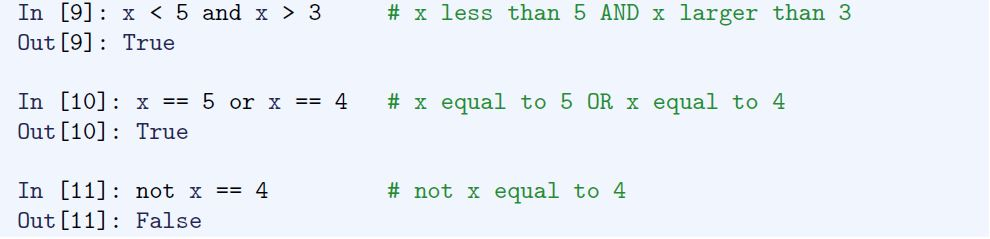
\includegraphics[width=0.9\textwidth]{figures/LLp47a}
\end{figure}

\begin{itemize}
	\item Boolean variable type
	\begin{itemize}
		\item int, float, str, \red{bool}
	\end{itemize}

	\item Boolean values may be combined into longer expressions by use of \texttt{and} and \texttt{or}
%	\item light touch: and, or, not but don't present truth tables %(??)--- refer back to lecture 1. Hmmm 
	\item basics of Boolean operators:~week 1 Thurs lecture
	\begin{itemize}
		\item covered in \emph{much} more depth in ELEC1710
	\end{itemize}
\end{itemize}

\end{frame}

%%==============================================================
%
%\begin{frame}[fragile]
%
%\frametitle{more Booleans---live demo}
%
%\begin{itemize}
%	\item xxx
%\end{itemize}
%
%\end{frame}

%==============================================================

\begin{frame}[fragile]

\frametitle{Example: Finding the Time of Flight}

\begin{itemize}
	\item context/description
	\item we modify/extend earlier example
\end{itemize}

%The Case Assume the ball is thrown with a slightly lower initial velocity, say
%4.5 ms−1, while everything else is kept unchanged. Since we still look at the first
%second of the flight, the heights at the end of the flight will then become negative.
%However, this only means that the ball has fallen below its initial starting position,
%i.e., the height where it left the hand, so there is nothing wrong with that. In an array
%y, we will then have a series of heights which towards the end of y become negative.
%As before, we will also have an array t with all the times for corresponding heights
%in y.

\end{frame}

%==============================================================

\begin{frame}[fragile]

\frametitle{Ball height vs.\ time}

\begin{figure}[ht]
	\centering
	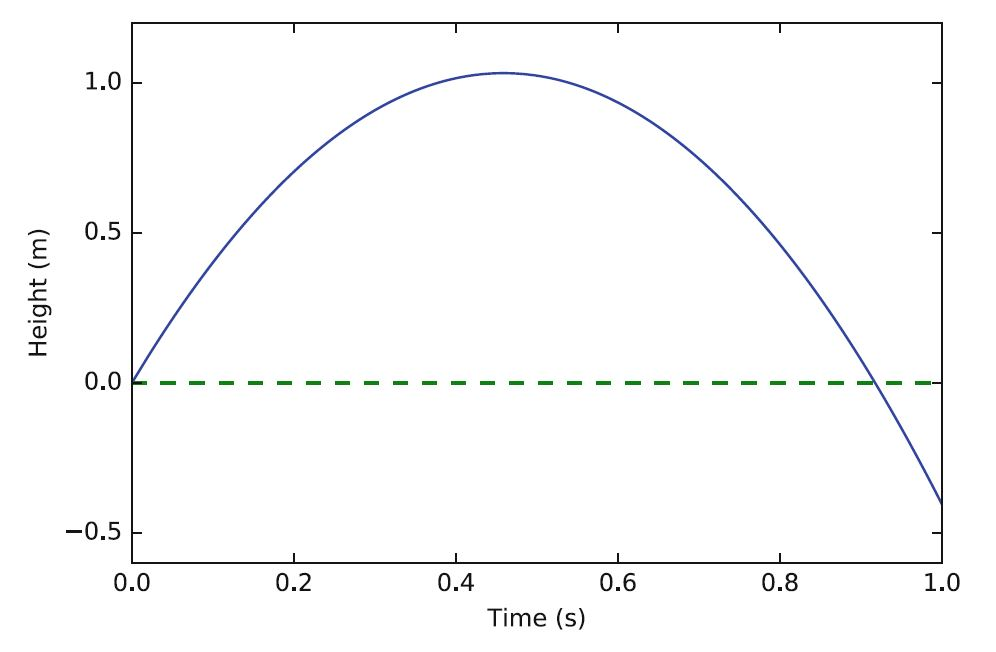
\includegraphics[width=0.9\textwidth]{figures/LLp66output}
\end{figure}

\end{frame}

%==============================================================

\begin{frame}[fragile]

\frametitle{}

\begin{figure}[ht]
	\centering
	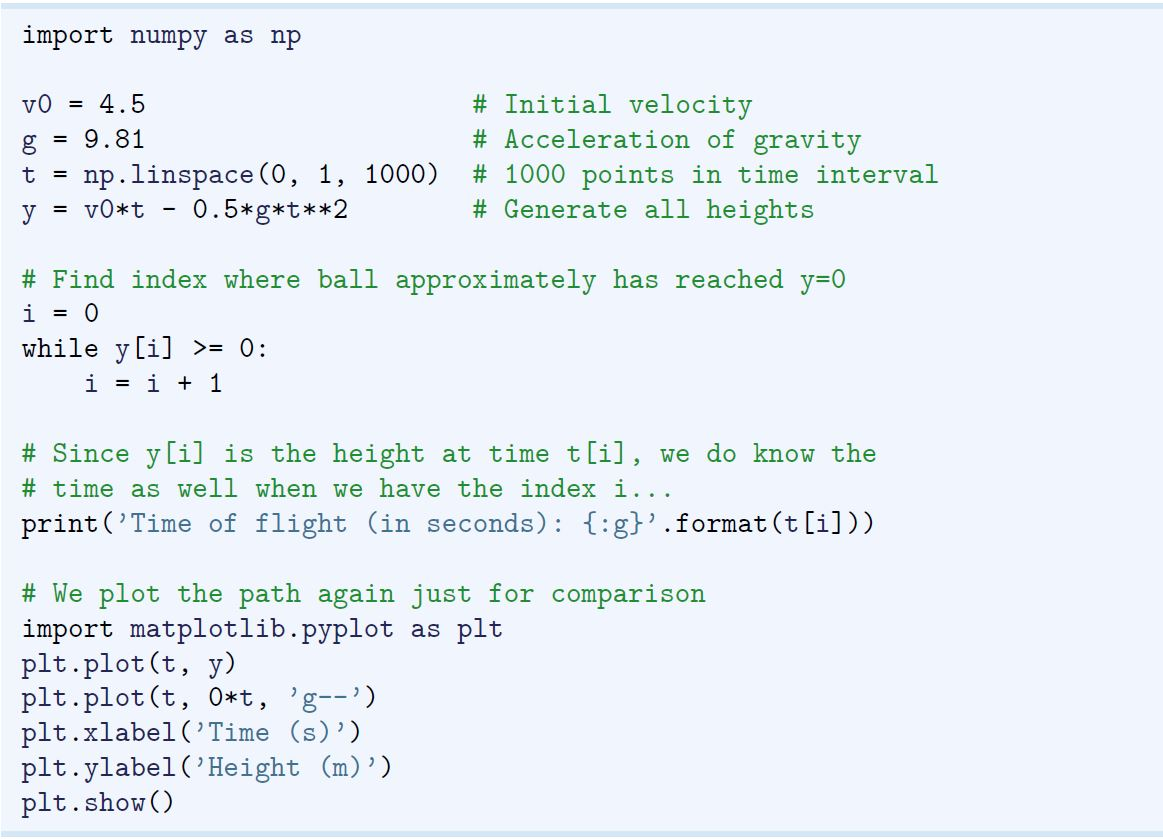
\includegraphics[width=0.9\textwidth]{figures/LLp65a}
\end{figure}
\vspace*{-3mm}
Python code:~\href{https://github.com/slgit/prog4comp_2/blob/master/py36-src/ball_time.py}{\texttt{ball\_time.py}}

\end{frame}

%==============================================================

\begin{frame}[fragile]

\frametitle{}

\begin{figure}[ht]
	\centering
	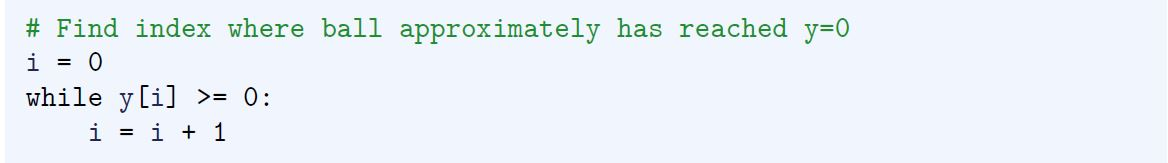
\includegraphics[width=\textwidth]{figures/LLp65b}
\end{figure}

\begin{itemize}
	\item slowly and meticulously consider y[i] \verb+>=+  condition
	\item index i after loop is index to first element of array that is negative
	\item confirm in Python
\end{itemize}

\end{frame}

%==============================================================

\begin{frame}[fragile]

\frametitle{}

\begin{figure}[ht]
	\centering
	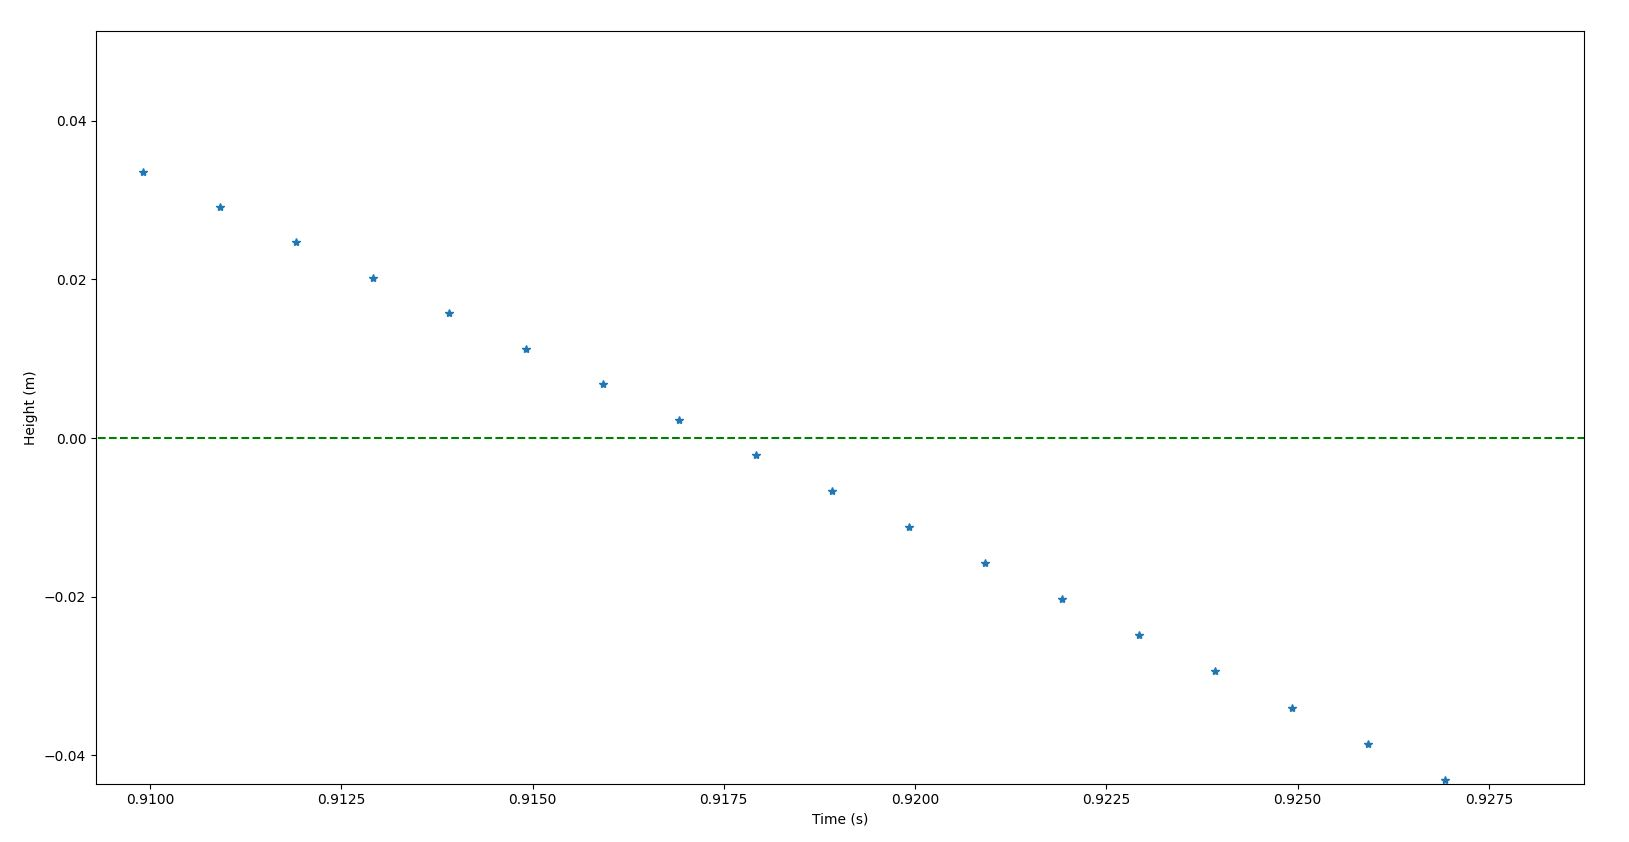
\includegraphics[width=\textwidth]{figures/LLp66ZoomOutput}
\end{figure}

\begin{itemize}
	\item plot as * then zoom in to see time where crossing occurs
\end{itemize}

\end{frame}

%==============================================================

\begin{frame}[fragile]

\frametitle{Structure of a typical \texttt{while} loop}

\begin{figure}[ht]
	\centering
	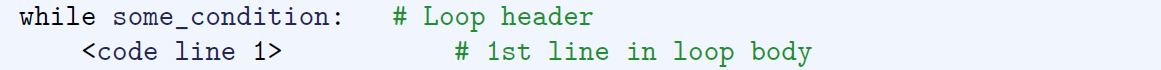
\includegraphics[width=\textwidth]{figures/LLp66a}
	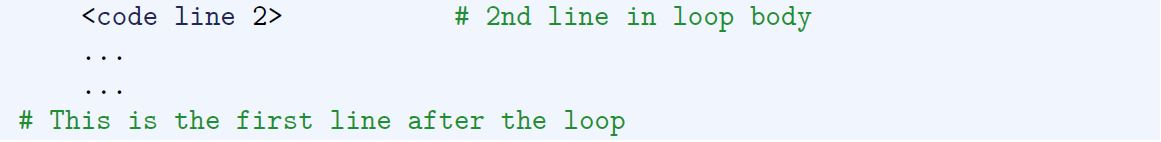
\includegraphics[width=\textwidth]{figures/LLp67a}
\end{figure}
\vspace*{-3mm}
\begin{itemize}
	\item first line is \red{\emph{while loop header}}
	\begin{itemize}
		\item reserved word \texttt{while}, ends with colon, both necessary
	\end{itemize}
	\item indented lines after header are a \red{\emph{block}} of statements%
	\begin{itemize}
		\item called the \red{\emph{loop body}}
	\end{itemize}
	\item indentation is 4 spaces by convention %---but \emph{some} indentation is necessary!
	\item once indentation is reversed, loop body has ended
\end{itemize}

%The first line here is the while loop header. It contains the reserved word while and
%ends with a colon, both are compulsory. The indented lines that follow the header
%(i.e., <code line 1>, <code line 2>, etc.) constitute a block of statements, the
%loop body. Indentation is done as with for loops, i.e., 4 spaces by convention. In
%our example above with the ball, there was only a single line in the loop body (i.e.,
%i = i + 1). As with for loops, one run-through of the loop body is referred to as
%an iteration. Once the indentation is reversed, the loop body has ended

\end{frame}

%==============================================================

\begin{frame}[fragile]

\frametitle{}

\begin{itemize}
	\item \texttt{some\_condition} is a Boolean expression
	\begin{itemize}
		\item must evaluate to \texttt{True} or \texttt{False}
	\end{itemize}
	
	\item[]
	
	\item if \texttt{some\_condition} is initially \texttt{False}:
	\begin{itemize}
		\item loop body statements are \emph{never} executed
	\end{itemize}

	\item[]
	
	\item if \texttt{some\_condition} is initially \texttt{True}:
	\begin{itemize}
		\item statements in loop body are evaluated once
		\item \texttt{some\_condition} evaluated again
		\item \ldots and the process continues
	\end{itemize}
	
	\item[]
	
	\item[] \textbf{Summary:}~\texttt{while} loop runs until the Boolean expression \texttt{some\_condition} becomes \texttt{False}
\end{itemize}

\end{frame}

%==============================================================

\begin{frame}[fragile]

\frametitle{Infinite Loops}

\begin{itemize}
	\item It is possible to have a while loop in which the condition never evaluates to False, meaning that program execution can not escape the loop!
	\item this is referred to as an infinite loop
\end{itemize}

\end{frame}

%%==============================================================
%
%\begin{frame}[fragile]
%
%\frametitle{Live demo: while loop}
%
%\end{frame}

%==============================================================

\begin{frame}[fragile]

\frametitle{$3)$ branching: if, elif and else)}

%Very often in life,5 and in computer programs, the next action depends on the
%outcome of a question starting with “if”. This gives the possibility of branching
%into different types of action depending on some criterion.
%As an introduction to branching, let us “build up” a little program that evaluates
%a water temperature provided by the program user.

\begin{itemize}
	\item context
	\item extended Example: Judging the Water Temperature %(need to change numbers!)
	\item will build up a program in stages
\end{itemize}

\end{frame}

%==============================================================

\begin{frame}[fragile]

\frametitle{One if-test}

\begin{itemize}
	\item screenshot/code LLp68
\end{itemize}

\end{frame}

%==============================================================

\begin{frame}[fragile]

\frametitle{Two if-tests}

\begin{itemize}
	\item LLp68
\end{itemize}

\end{frame}

%==============================================================

\begin{frame}[fragile]

\frametitle{An if-else Construction}

\begin{itemize}
	\item LLp69
\end{itemize}

\end{frame}

%==============================================================

\begin{frame}[fragile]

\frametitle{An if-elif-else Construction}

\begin{itemize}
	\item LLp69
\end{itemize}

\end{frame}

%==============================================================

\begin{frame}[fragile]

\frametitle{general form of an if-elif-else}

\begin{itemize}
	\item \S3.3.2
\end{itemize}

\end{frame}

%==============================================================

\begin{frame}[fragile]

\frametitle{branching summary}

\begin{itemize}
	\item if
	\item if / else
	\item if / elif / else
\end{itemize}

\end{frame}

%%==============================================================
%
%\begin{frame}[fragile]
%
%\frametitle{Example: Finding the Maximum Height}
%
%\begin{itemize}
%	\item excellent illustration of further mod to ball plot
%	\item \textbf{but save this for Thursday lecture}
%	\item can solve in two ways: both shown on p71
%\end{itemize}
%
%\end{frame}

%%==============================================================
%
%\begin{frame}[fragile]
%
%\frametitle{}
%
%\begin{itemize}
%	\item xxx
%\end{itemize}
%
%\end{frame}

%%==============================================================
%
%\begin{frame}[fragile]
%
%\frametitle{Live demo: branching}
%
%\end{frame}

%==============================================================

\begin{frame}[fragile]

\frametitle{Lecture summary}

%% https://www.overleaf.com/learn/latex/code_listing
%
%\begin{lstlisting}[language=Python]
%import numpy as np
%    
%def incmatrix(genl1,genl2):
%    m = len(genl1)
%    n = len(genl2)
%    M = None #to become the incidence matrix
%    VT = np.zeros((n*m,1), int)  #dummy variable
%    
%    #compute the bitwise xor matrix
%    M1 = bitxormatrix(genl1)
%    M2 = np.triu(bitxormatrix(genl2),1) 
%
%    for i in range(m-1):
%        for j in range(i+1, m):
%            [r,c] = np.where(M2 == M1[i,j])
%            for k in range(len(r)):
%                VT[(i)*n + r[k]] = 1;
%                VT[(i)*n + c[k]] = 1;
%                VT[(j)*n + r[k]] = 1;
%                VT[(j)*n + c[k]] = 1;
%                
%                if M is None:
%                    M = np.copy(VT)
%                else:
%                    M = np.concatenate((M, VT), 1)
%                
%                VT = np.zeros((n*m,1), int)
%    
%    return M
%\end{lstlisting}

\end{frame}

\end{document}